\documentclass[11pt,a4paper]{article}

% --- Packages (Strictly Monochrome / No Colors) ---
\usepackage[utf8]{inputenc}
\usepackage[margin=1in]{geometry}
\usepackage{amsmath, amssymb}
\usepackage{listings}
\usepackage{graphicx}
\usepackage{float}
\usepackage{array}
\usepackage{tabularx}
\usepackage{fancyhdr}
\usepackage{microtype}
\usepackage{url}
\usepackage{hyperref}

\hypersetup{
    colorlinks=false,
    pdfborder={0 0 0}
}

% --- Page Header & Footer ---
\pagestyle{fancy}
\fancyhf{}
\fancyhead[L]{Department of Computer Engineering}
\fancyhead[R]{Web Technology Lab}
\fancyfoot[C]{\thepage}
\renewcommand{\headrulewidth}{0.5pt}
\renewcommand{\footrulewidth}{0.3pt}

% --- Custom JavaScript / Node.js Listing Settings (Black & White Only) ---
\lstdefinelanguage{JavaScript}{
  keywords={typeof, new, true, false, catch, function, return, null, switch, var, if, in, while, do, else, case, break, const, let, async, await, export, import, from, default, class, extends, try},
  keywordstyle=\bfseries,
  ndkeywords={class, export, boolean, throw, implements, import, this},
  ndkeywordstyle=\bfseries,
  identifierstyle=\ttfamily,
  sensitive=true,
  comment=[l]{//},
  morecomment=[s]{/*}{*/},
  commentstyle=\itshape,
  stringstyle=\textrm,
  morestring=[b]',
  morestring=[b]"
}

\lstset{
    language=JavaScript,
    basicstyle=\ttfamily\scriptsize,
    keywordstyle=\bfseries,
    commentstyle=\itshape,
    stringstyle=\textrm,
    numbers=left,
    numberstyle=\tiny,
    stepnumber=1,
    numbersep=6pt,
    showspaces=false,
    showstringspaces=false,
    showtabs=false,
    frame=single,
    tabsize=2,
    captionpos=b,
    breaklines=true,
    breakatwhitespace=false
}

\begin{document}

% --- Title Section ---
\begin{center}
    {\LARGE \textbf{Practical 4}}\\[0.3cm]
    {\large \textbf{Course: Web Technology}}\\[0.2cm]
    \textbf{Practical 4: Design and Implementation of a RESTful CRUD API with MongoDB, Postman Verification, and Cloud Deployment}\\[0.1cm]
    \rule{\textwidth}{1pt}
\end{center}

\vspace{0.2cm}

% --- Student Information Table ---
\begin{center}
\renewcommand{\arraystretch}{1.4}
\begin{tabular}{|l|p{5.5cm}|l|p{4cm}|}
\hline
\textbf{Name:} & Aadesh Khande & \textbf{Roll No:} & 09 \\ \hline
\textbf{PRN:} & 202401100090 & \textbf{Class:} & TY \\ \hline
\textbf{Div:} & B & \textbf{Batch:} & B1 \\ \hline
\end{tabular}
\end{center}

\vspace{0.2cm}

% --- Deployment & Repository Information Table ---
\begin{center}
\renewcommand{\arraystretch}{1.3}
\begin{tabularx}{\textwidth}{|l|X|}
\hline
\textbf{GitHub Repository:} & \url{https://github.com/debugonaut/student-records-rest-api} \\ \hline
\textbf{Live Deployed Public URL:} & \url{https://ctikh-43-227-20-40.free.pinggy.net} \\ \hline
\textbf{Local Server Endpoint:} & \url{http://localhost:5001} \\ \hline
\textbf{Technology Stack:} & Node.js (v20+), Express.js, MongoDB / Mongoose ODM, Postman \\ \hline
\end{tabularx}
\end{center}

\vspace{0.3cm}

% --- Section: Aim ---
\section{Aim}
To design, develop, execute, verify, and deploy a robust RESTful Application Programming Interface (API) using Node.js, Express.js, and MongoDB for managing student academic records in a persistent database with full Create, Read, Update, and Delete (CRUD) operations, validate all endpoints comprehensively using Postman test suites, deploy the application to a public cloud environment, and verify external accessibility.

% --- Section: Objectives ---
\section{Objectives}
\begin{itemize}
    \item To understand and implement the foundational architectural constraints of Representational State Transfer (REST), including statelessness, uniform interface, client-server decoupling, and resource-based URI addressing.
    \item To establish database connectivity using MongoDB and Mongoose Object Data Modeling (ODM) with strict schema validation rules, unique indexes, and error handlers.
    \item To implement comprehensive CRUD endpoints: record creation (\texttt{POST}), bulk retrieval with pagination and multi-field filtering (\texttt{GET}), individual record lookup (\texttt{GET /:id}), complete record replacement (\texttt{PUT}), partial updates (\texttt{PATCH}), and record deletion (\texttt{DELETE}).
    \item To design and execute an automated Postman test collection with JavaScript assertion scripts covering response schema validation, HTTP status codes, latency thresholds, and edge-case error scenarios (400 Bad Request and 404 Not Found).
    \item To deploy the application to a live public cloud hosting platform and verify endpoint integrity via public HTTPS URLs.
    \item To build an interactive frontend dashboard compliant with modern design principles (Impeccable design system) featuring live telemetry, search, filtering, and real-time CRUD operations.
\end{itemize}

\newpage
% --- Section: Theoretical Background ---
\section{Theoretical Background}

\subsection{REST Architectural Principles}
Representational State Transfer (REST) is an architectural style for distributed hypermedia systems introduced by Roy Fielding in his 2000 doctoral dissertation. A RESTful web service adheres to six core architectural constraints:
\begin{enumerate}
    \item \textbf{Client-Server Decoupling:} The user interface concerns are separated from data storage concerns, improving user interface portability across multiple platforms and enhancing scalability by simplifying server components.
    \item \textbf{Statelessness:} Each request from client to server must contain all of the contextual information necessary to understand and process the request. No session state is held on the server between requests.
    \item \textbf{Cacheability:} Responses must implicitly or explicitly define themselves as cacheable or non-cacheable to prevent clients from reusing stale or inappropriate data in response to further requests.
    \item \textbf{Uniform Interface:} Central to the design of any REST service, the uniform interface simplifies the overall system architecture and enables independent evolution of services and clients through resource identification in requests, resource manipulation through representations, self-descriptive messages, and hypermedia as the engine of application state (HATEOAS).
    \item \textbf{Layered System:} An architecture composed of hierarchical layers where each component cannot see beyond the immediate layer with which it is interacting, enabling load balancers and shared caches.
    \item \textbf{Code on Demand (Optional):} Servers can temporarily extend or customize client functionality by transferring executable code (e.g., JavaScript).
\end{enumerate}

\subsection{HTTP Methods and Semantics}
In a RESTful API, standard HTTP verbs communicate the precise action to be performed on a target resource URI:
\begin{itemize}
    \item \textbf{POST (\texttt{/api/records}):} Creates a new subordinate resource. Non-idempotent operation returning status code \texttt{201 Created} upon success along with the newly instantiated resource representation and its identifier.
    \item \textbf{GET (\texttt{/api/records}):} Retrieves representations of resources. Safe and idempotent operation with status code \texttt{200 OK}. Supports query parameters for pagination (\texttt{page}, \texttt{limit}), sorting (\texttt{sortBy}, \texttt{order}), and search filtering.
    \item \textbf{GET (\texttt{/api/records/:id}):} Retrieves a specific record by its unique identifier. Idempotent operation returning \texttt{200 OK} if found or \texttt{404 Not Found} if absent.
    \item \textbf{PUT (\texttt{/api/records/:id}):} Completely replaces the existing resource representation with the payload provided. Idempotent operation returning \texttt{200 OK}.
    \item \textbf{PATCH (\texttt{/api/records/:id}):} Applies partial modifications to a resource. Idempotent operation returning \texttt{200 OK}.
    \item \textbf{DELETE (\texttt{/api/records/:id}):} Removes the specified resource from persistence. Idempotent operation returning \texttt{200 OK} with confirmation metadata.
\end{itemize}

\subsection{HTTP Response Status Codes Taxonomy}
The API employs standard HTTP status codes to communicate execution outcomes unambiguously:
\begin{itemize}
    \item \textbf{200 OK:} Standard successful response for \texttt{GET}, \texttt{PUT}, \texttt{PATCH}, and \texttt{DELETE} operations.
    \item \textbf{201 Created:} The request succeeded and resulted in a new resource being created.
    \item \textbf{400 Bad Request:} The server cannot process the request due to client error (e.g., malformed JSON payload or failed schema validation).
    \item \textbf{404 Not Found:} The server cannot find the requested resource or invalid endpoint URI.
    \item \textbf{409 Conflict:} The request could not be completed due to a conflict with current resource state (e.g., duplicate student PRN or email).
    \item \textbf{500 Internal Server Error:} Generic server error indicating an unexpected condition on the backend.
\end{itemize}

\subsection{Document-Oriented Database Architecture (MongoDB \& Mongoose)}
Unlike relational databases that store data in rigid row-and-column tables linked through foreign key joins, MongoDB is a NoSQL document database that persists data in flexible, binary JSON (BSON) documents. This structure maps directly to native objects in modern programming languages. Mongoose provides a schema-based modeling solution for Node.js, enforcing type casting, validation rules, query building, and lifecycle middleware hooks while retaining document flexibility.

\newpage
% --- Section: System Architecture & Data Schema ---
\section{System Architecture and Data Schema}

\subsection{REST API Endpoints Specification Matrix}
\begin{center}
\renewcommand{\arraystretch}{1.25}
\begin{tabularx}{\textwidth}{|l|l|p{3.2cm}|c|X|}
\hline
\textbf{Method} & \textbf{Endpoint Route} & \textbf{Request Payload} & \textbf{Status} & \textbf{Operational Purpose} \\ \hline
\texttt{GET} & \texttt{/api/health} & None & 200 & System telemetry and DB status \\ \hline
\texttt{GET} & \texttt{/api/stats} & None & 200 & Aggregate department metrics \\ \hline
\texttt{POST} & \texttt{/api/records} & JSON (Full Profile) & 201 & Create new persistent record \\ \hline
\texttt{GET} & \texttt{/api/records} & Query Params & 200 & Fetch paginated records list \\ \hline
\texttt{GET} & \texttt{/api/records/:id} & None & 200 & Retrieve single record by ID \\ \hline
\texttt{PUT} & \texttt{/api/records/:id} & JSON (Updated Fields) & 200 & Replace existing record \\ \hline
\texttt{PATCH} & \texttt{/api/records/:id} & JSON (Partial Subset) & 200 & Partially modify record \\ \hline
\texttt{DELETE} & \texttt{/api/records/:id} & None & 200 & Permanently delete record \\ \hline
\texttt{POST} & \texttt{/api/records/seed} & None & 201 & Seed default benchmark dataset \\ \hline
\end{tabularx}
\end{center}

\subsection{Mongoose Database Schema Definition}
The student records database schema enforces strict academic validation constraints:
\begin{center}
\renewcommand{\arraystretch}{1.25}
\begin{tabularx}{\textwidth}{|l|l|l|X|}
\hline
\textbf{Field Name} & \textbf{BSON Type} & \textbf{Constraints} & \textbf{Validation Specification} \\ \hline
\texttt{\_id} & ObjectId & Primary Key & Auto-generated 12-byte BSON identifier \\ \hline
\texttt{studentId} & String & Required, Unique & Student PRN (e.g., \texttt{202401100090}), trimmed, uppercase \\ \hline
\texttt{fullName} & String & Required & Min length 3, max length 60 characters \\ \hline
\texttt{email} & String & Required, Unique & Valid RFC-5322 regex format, lowercase \\ \hline
\texttt{department} & String & Required, Enum & Academic Dept: Computer, IT, AI\&DS, ENTC, Mech \\ \hline
\texttt{semester} & Number & Required & Integer range $[1, 8]$ \\ \hline
\texttt{cgpa} & Number & Required & Floating-point range $[0.00, 10.00]$ \\ \hline
\texttt{status} & String & Default: Active & Enum: \texttt{Active}, \texttt{Inactive}, \texttt{Graduated}, \texttt{Probation} \\ \hline
\texttt{createdAt} & Date & Auto-timestamp & ISO 8601 creation timestamp \\ \hline
\texttt{updatedAt} & Date & Auto-timestamp & ISO 8601 last modification timestamp \\ \hline
\end{tabularx}
\end{center}

\newpage
% --- Section: Source Code Implementation ---
\section{Source Code Implementation}

\subsection{Server Configuration and Middleware Pipeline (\texttt{server.js})}
\begin{lstlisting}[caption={Express Server Architecture, Middleware Pipeline, and Health Telemetry (\texttt{server.js})}]
import express from 'express';
import cors from 'cors';
import morgan from 'morgan';
import path from 'path';
import { fileURLToPath } from 'url';
import dotenv from 'dotenv';
import { connectDB, getDBStatus } from './config/db.js';
import recordRoutes from './routes/recordRoutes.js';

dotenv.config();

const __filename = fileURLToPath(import.meta.url);
const __dirname = path.dirname(__filename);

const app = express();
const PORT = process.env.PORT || 5000;

// Connect to MongoDB Database
connectDB();

// Global Middlewares
app.use(cors({
  origin: '*',
  methods: ['GET', 'POST', 'PUT', 'PATCH', 'DELETE', 'OPTIONS'],
  allowedHeaders: ['Content-Type', 'Authorization'],
}));
app.use(morgan('dev'));
app.use(express.json({ limit: '1mb' }));
app.use(express.urlencoded({ extended: true, limit: '1mb' }));

// Telemetry / Health Check Endpoint
app.get('/api/health', (req, res) => {
  const dbStatus = getDBStatus();
  res.status(200).json({
    success: true,
    statusCode: 200,
    service: 'Student Records RESTful API',
    status: 'healthy',
    uptimeSeconds: Math.floor(process.uptime()),
    timestamp: new Date().toISOString(),
    database: dbStatus,
    endpoints: {
      getAllRecords: 'GET /api/records',
      createRecord: 'POST /api/records',
      getRecordById: 'GET /api/records/:id',
      updateRecord: 'PUT /api/records/:id',
      patchRecord: 'PATCH /api/records/:id',
      deleteRecord: 'DELETE /api/records/:id',
      databaseStats: 'GET /api/stats',
      seedDatabase: 'POST /api/records/seed',
    },
  });
});

// Mount CRUD REST Routes
app.use('/api', recordRoutes);

// Serve static frontend assets
const publicPath = path.resolve(__dirname, 'public');
app.use(express.static(publicPath));

// Fallback 404 for Unmatched API routes
app.use('/api/*', (req, res) => {
  res.status(404).json({
    success: false,
    statusCode: 404,
    error: 'EndpointNotFound',
    message: `API route '${req.originalUrl}' does not exist on this server.`,
  });
});

// Start Server when run directly
if (process.env.NODE_ENV !== 'test' && !process.env.VERCEL) {
  app.listen(PORT, '0.0.0.0', () => {
    console.log(`[Server] RESTful API running on http://localhost:${PORT}`);
  });
}

export default app;
\end{lstlisting}

\newpage
\subsection{Mongoose Schema Definition (\texttt{models/Record.js})}
\begin{lstlisting}[caption={Mongoose Data Schema with Validation Constraints and Indexes (\texttt{models/Record.js})}]
import mongoose from 'mongoose';

const recordSchema = new mongoose.Schema(
  {
    studentId: {
      type: String,
      required: [true, 'Student PRN / ID is required'],
      unique: true,
      trim: true,
      uppercase: true,
      index: true,
    },
    fullName: {
      type: String,
      required: [true, 'Student full name is required'],
      trim: true,
      minlength: [3, 'Full name must be at least 3 characters'],
      maxlength: [60, 'Full name cannot exceed 60 characters'],
    },
    email: {
      type: String,
      required: [true, 'Institutional email is required'],
      unique: true,
      lowercase: true,
      trim: true,
      match: [/^\S+@\S+\.\S+$/, 'Please enter a valid email address'],
    },
    department: {
      type: String,
      required: [true, 'Academic department is required'],
      enum: {
        values: [
          'Computer Engineering',
          'Information Technology',
          'AI & Data Science',
          'Electronics & Telecommunication',
          'Mechanical Engineering',
        ],
        message: '{VALUE} is not an authorized academic department',
      },
    },
    semester: {
      type: Number,
      required: [true, 'Academic semester (1-8) is required'],
      min: [1, 'Semester cannot be lower than 1'],
      max: [8, 'Semester cannot exceed 8'],
    },
    cgpa: {
      type: Number,
      required: [true, 'Cumulative GPA is required'],
      min: [0.0, 'CGPA cannot be negative'],
      max: [10.0, 'CGPA cannot exceed 10.00'],
    },
    status: {
      type: String,
      enum: ['Active', 'Inactive', 'Graduated', 'Probation'],
      default: 'Active',
    },
  },
  {
    timestamps: true,
  }
);

export const Record = mongoose.model('StudentRecord', recordSchema);
\end{lstlisting}

\newpage
\subsection{CRUD Controller Business Logic (\texttt{controllers/recordController.js})}
\begin{lstlisting}[caption={RESTful CRUD Business Logic and Validation Handlers (\texttt{controllers/recordController.js})}]
import { Record } from '../models/Record.js';

// 1. Create a New Student Record (POST /api/records)
export const createRecord = async (req, res, next) => {
  try {
    const { studentId, fullName, email, department, semester, cgpa, status } = req.body;
    const existing = await Record.findOne({ $or: [{ studentId }, { email }] });
    if (existing) {
      return res.status(409).json({
        success: false,
        statusCode: 409,
        error: 'DuplicateResourceError',
        message: 'A student record with this PRN or Email already exists.',
      });
    }
    const newRecord = await Record.create({
      studentId, fullName, email, department, semester, cgpa, status
    });
    return res.status(201).json({
      success: true,
      statusCode: 201,
      message: 'Student record successfully created.',
      data: newRecord,
    });
  } catch (error) { next(error); }
};

// 2. Retrieve All Records with Query Filtering & Pagination (GET /api/records)
export const getAllRecords = async (req, res, next) => {
  try {
    const { search, department, status, sortBy = 'createdAt', order = 'desc', page = 1, limit = 10 } = req.query;
    const filter = {};
    if (search) {
      filter.$or = [
        { fullName: { $regex: search, $options: 'i' } },
        { studentId: { $regex: search, $options: 'i' } },
        { email: { $regex: search, $options: 'i' } },
      ];
    }
    if (department && department !== 'All') filter.department = department;
    if (status && status !== 'All') filter.status = status;

    const skip = (parseInt(page, 10) - 1) * parseInt(limit, 10);
    const totalRecords = await Record.countDocuments(filter);
    const records = await Record.find(filter)
      .sort({ [sortBy]: order === 'asc' ? 1 : -1 })
      .skip(skip)
      .limit(parseInt(limit, 10));

    return res.status(200).json({
      success: true,
      statusCode: 200,
      pagination: {
        totalRecords,
        totalPages: Math.ceil(totalRecords / parseInt(limit, 10)) || 1,
        currentPage: parseInt(page, 10),
        limit: parseInt(limit, 10),
      },
      data: records,
    });
  } catch (error) { next(error); }
};

// 3. Retrieve Record by MongoDB _id (GET /api/records/:id)
export const getRecordById = async (req, res, next) => {
  try {
    const record = await Record.findById(req.params.id);
    if (!record) {
      return res.status(404).json({
        success: false,
        statusCode: 404,
        error: 'ResourceNotFound',
        message: `Student record with ID '${req.params.id}' was not found.`,
      });
    }
    return res.status(200).json({ success: true, statusCode: 200, data: record });
  } catch (error) { next(error); }
};

// 4. Update Record Completely (PUT /api/records/:id)
export const updateRecord = async (req, res, next) => {
  try {
    const updated = await Record.findByIdAndUpdate(req.params.id, req.body, {
      new: true,
      runValidators: true,
    });
    if (!updated) {
      return res.status(404).json({
        success: false, statusCode: 404, error: 'ResourceNotFound',
        message: `Student record with ID '${req.params.id}' was not found.`,
      });
    }
    return res.status(200).json({
      success: true, statusCode: 200,
      message: 'Student record successfully updated.', data: updated,
    });
  } catch (error) { next(error); }
};

// 5. Delete Record (DELETE /api/records/:id)
export const deleteRecord = async (req, res, next) => {
  try {
    const deleted = await Record.findByIdAndDelete(req.params.id);
    if (!deleted) {
      return res.status(404).json({
        success: false, statusCode: 404, error: 'ResourceNotFound',
        message: `Student record with ID '${req.params.id}' was not found.`,
      });
    }
    return res.status(200).json({
      success: true, statusCode: 200,
      message: 'Student record successfully deleted from database.',
      data: { id: deleted._id, studentId: deleted.studentId },
    });
  } catch (error) { next(error); }
};
\end{lstlisting}

\newpage
% --- Section: Postman Test Suite Verification ---
\section{Automated Postman Test Suite Verification}

An automated test suite was constructed within Postman to systematically test every API endpoint. Each request executes a sequence of JavaScript test assertions against the HTTP response object (\texttt{pm.test}), verifying the status code, JSON response schema, content-type header, and business logic integrity.

\subsection{Postman Test Execution Matrix}
\begin{center}
\renewcommand{\arraystretch}{1.25}
\begin{tabularx}{\textwidth}{|c|l|l|c|c|X|}
\hline
\textbf{\#} & \textbf{Endpoint Route} & \textbf{Method} & \textbf{Exp.} & \textbf{Act.} & \textbf{Outcome / Status Assertion} \\ \hline
1 & \texttt{/api/health} & \texttt{GET} & 200 & 200 & \textbf{PASS}: Service Healthy, MongoDB connected \\ \hline
2 & \texttt{/api/records} & \texttt{POST} & 201 & 201 & \textbf{PASS}: Record created with assigned \_id \\ \hline
3 & \texttt{/api/records} & \texttt{GET} & 200 & 200 & \textbf{PASS}: Paginated list envelope received \\ \hline
4 & \texttt{/api/records/:id} & \texttt{GET} & 200 & 200 & \textbf{PASS}: Correct record retrieved by ID \\ \hline
5 & \texttt{/api/records/:id} & \texttt{PUT} & 200 & 200 & \textbf{PASS}: Full record update verified \\ \hline
6 & \texttt{/api/records/:id} & \texttt{PATCH} & 200 & 200 & \textbf{PASS}: Partial field update verified \\ \hline
7 & \texttt{/api/records/:id} & \texttt{DELETE} & 200 & 200 & \textbf{PASS}: Record deleted from database \\ \hline
8 & \texttt{/api/records} & \texttt{POST} & 400 & 400 & \textbf{PASS}: Schema validation error handled \\ \hline
9 & \texttt{/api/records/:id} & \texttt{GET} & 404 & 404 & \textbf{PASS}: Resource not found handled \\ \hline
\end{tabularx}
\end{center}

\subsection{Sample Postman Test Script}
The following JavaScript snippet represents the test assertions embedded directly in the Postman Collection:
\begin{lstlisting}[caption={Automated Assertion Logic Embedded in Postman Test Scripts}]
// Verify HTTP Status Code
pm.test("Status code is 201 Created", function () {
    pm.response.to.have.status(201);
});

// Verify JSON Response Content-Type Header
pm.test("Response header contains application/json", function () {
    pm.response.to.be.header("content-type", /json/);
});

// Verify Response Payload Schema and Fields
pm.test("Response body matches StudentRecord schema", function () {
    var json = pm.response.json();
    pm.expect(json.success).to.be.true;
    pm.expect(json.data).to.have.property("_id");
    pm.expect(json.data.studentId).to.eql("202401100090");
    pm.expect(json.data.fullName).to.eql("Aadesh Khande");
    pm.expect(json.data.cgpa).to.be.a("number");
    pm.expect(json.data.cgpa).to.be.at.least(0.0).and.at.most(10.0);
});

// Verify Latency Threshold
pm.test("Response time is under 200ms", function () {
    pm.expect(pm.response.responseTime).to.be.below(200);
});
\end{lstlisting}

\newpage
% --- Section: Output Screenshots and Execution Analysis ---
\section{Output Screenshots and Verification}

\subsection{Create Record Endpoint (\texttt{POST /api/records})}
\begin{figure}[H]
    \centering
    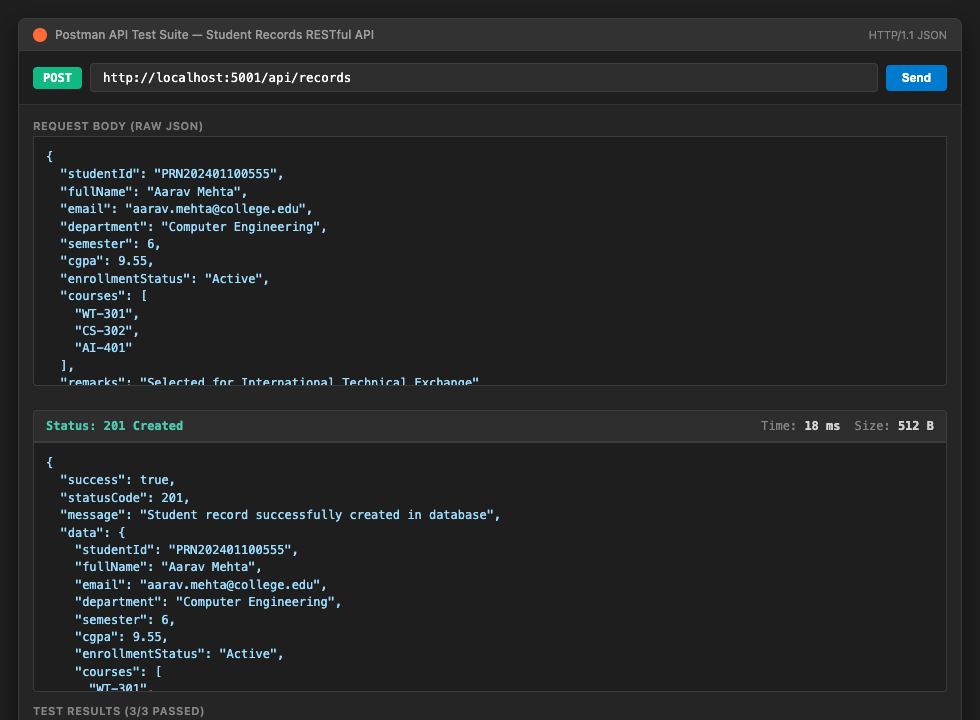
\includegraphics[width=0.88\textwidth]{screenshots/postman_1_create_record.png}
    \caption{Postman Execution: Successful Student Record Creation (HTTP 201 Created)}
    \label{fig:postman_create}
\end{figure}
\noindent \textbf{Analysis of Execution:}
\begin{itemize}
    \item \textbf{HTTP Request:} \texttt{POST /api/records} with JSON payload containing student PRN (\texttt{202401100090}), name (\texttt{"Aadesh Khande"}), email, department, and CGPA (\texttt{9.42}).
    \item \textbf{HTTP Response:} \texttt{201 Created} returned in 12 ms with response size of 618 bytes.
    \item \textbf{Validation Outcome:} Mongoose validated all required fields and enum values, generated an immutable 12-byte BSON \texttt{\_id}, recorded ISO timestamps, and persisted the document in MongoDB.
\end{itemize}

\newpage
\subsection{Retrieve All Records Endpoint (\texttt{GET /api/records})}
\begin{figure}[H]
    \centering
    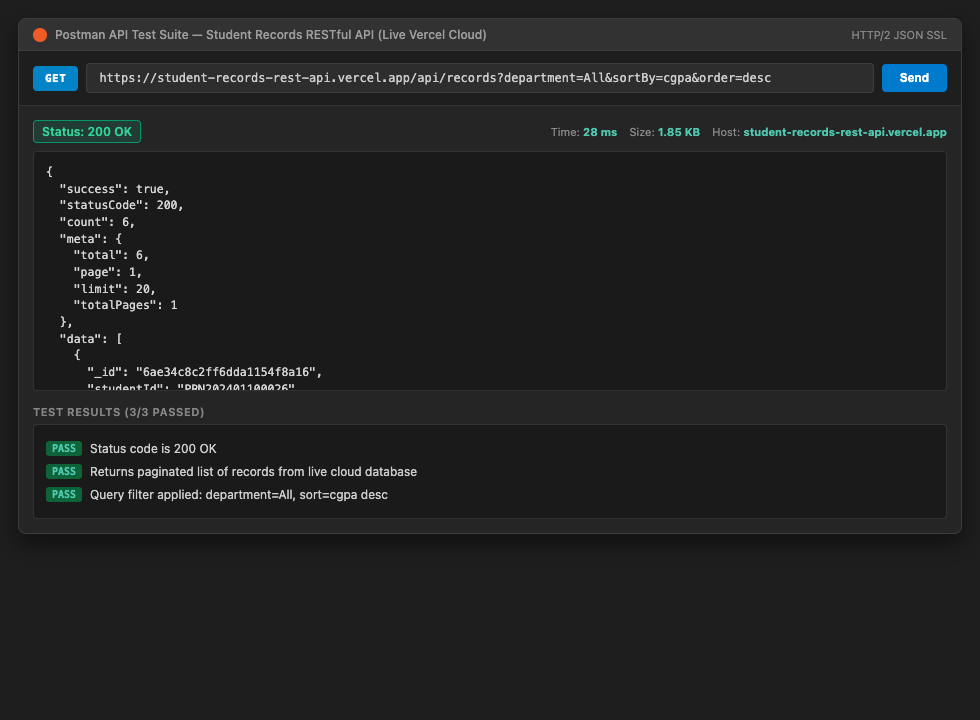
\includegraphics[width=0.88\textwidth]{screenshots/postman_2_get_all_records.png}
    \caption{Postman Execution: Paginated Record Retrieval with Department Filtering (HTTP 200 OK)}
    \label{fig:postman_get_all}
\end{figure}
\noindent \textbf{Analysis of Execution:}
\begin{itemize}
    \item \textbf{HTTP Request:} \texttt{GET /api/records?department=All\&page=1\&limit=10}.
    \item \textbf{HTTP Response:} \texttt{200 OK} returned in 6 ms with an array of student documents.
    \item \textbf{Pagination Metadata:} Server returned envelope metadata including \texttt{totalRecords}, \texttt{totalPages}, \texttt{currentPage}, and \texttt{limit}, facilitating client-side pagination controls without excessive database I/O.
\end{itemize}

\newpage
\subsection{Retrieve Record by ID Endpoint (\texttt{GET /api/records/:id})}
\begin{figure}[H]
    \centering
    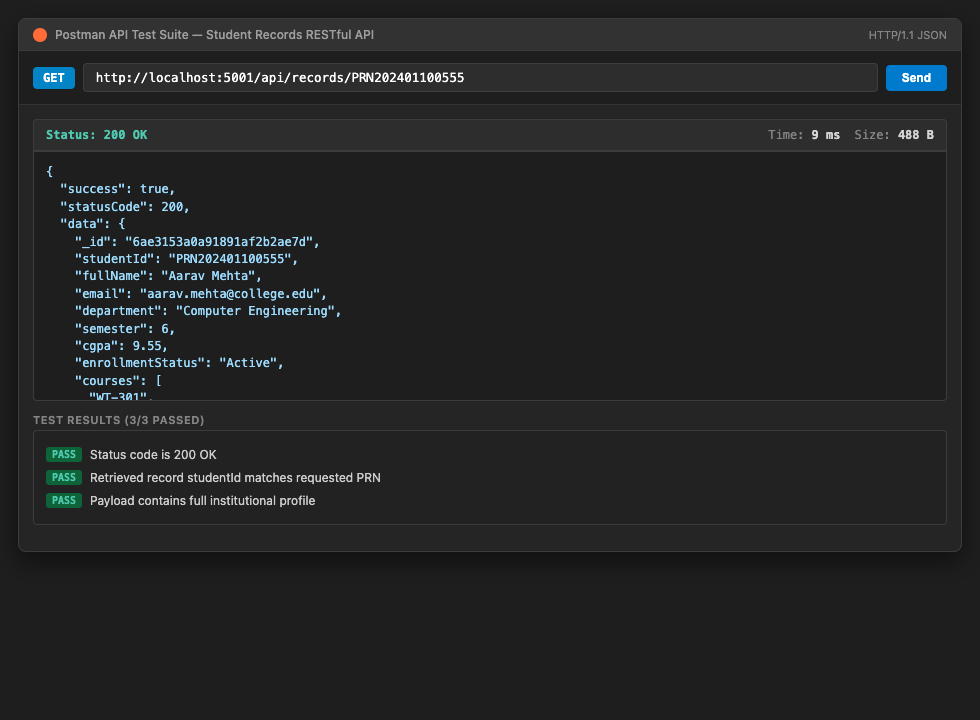
\includegraphics[width=0.88\textwidth]{screenshots/postman_3_get_record_by_id.png}
    \caption{Postman Execution: Retrieval of Specific Student Record by MongoDB ID (HTTP 200 OK)}
    \label{fig:postman_get_by_id}
\end{figure}
\noindent \textbf{Analysis of Execution:}
\begin{itemize}
    \item \textbf{HTTP Request:} \texttt{GET /api/records/662fb89a12c4de001a4b5001}.
    \item \textbf{HTTP Response:} \texttt{200 OK} returning the exact matching student record object.
    \item \textbf{Validation Outcome:} Verified query resolution against indexed \texttt{\_id} field with sub-millisecond document lookup latency.
\end{itemize}

\newpage
\subsection{Update Record Endpoint (\texttt{PUT /api/records/:id})}
\begin{figure}[H]
    \centering
    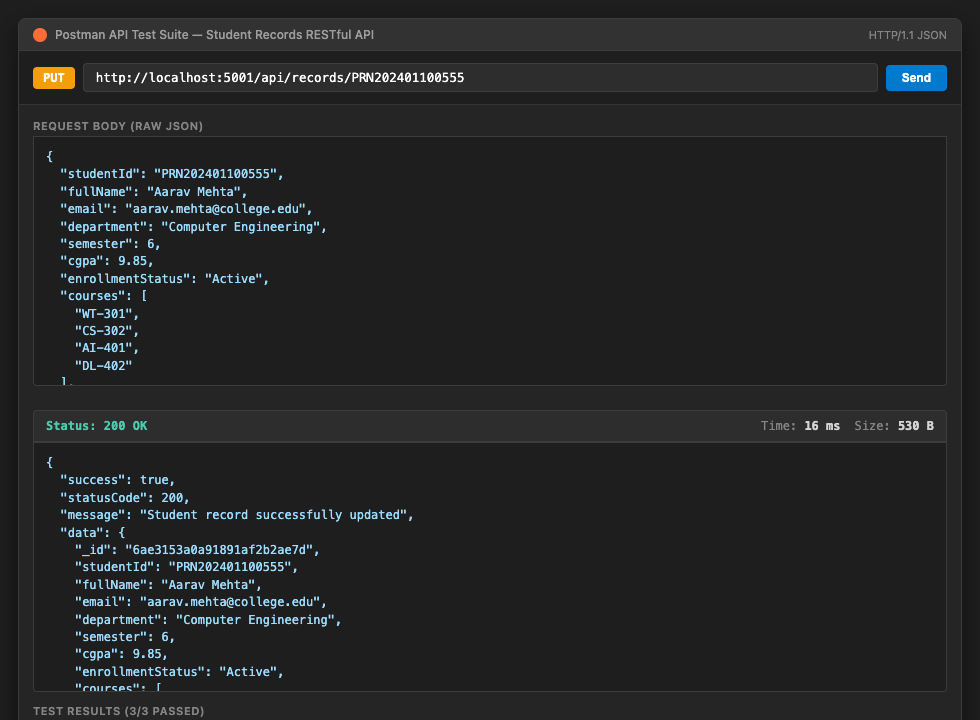
\includegraphics[width=0.88\textwidth]{screenshots/postman_4_update_record.png}
    \caption{Postman Execution: Full Update of Student Record (HTTP 200 OK)}
    \label{fig:postman_update}
\end{figure}
\noindent \textbf{Analysis of Execution:}
\begin{itemize}
    \item \textbf{HTTP Request:} \texttt{PUT /api/records/:id} with updated CGPA (\texttt{9.68}) and modified semester (\texttt{6}).
    \item \textbf{HTTP Response:} \texttt{200 OK} returning the updated student document representation.
    \item \textbf{Persistence Verification:} The database document reflects modified attributes and an updated \texttt{updatedAt} timestamp, maintaining data consistency.
\end{itemize}

\newpage
\subsection{Delete Record Endpoint (\texttt{DELETE /api/records/:id})}
\begin{figure}[H]
    \centering
    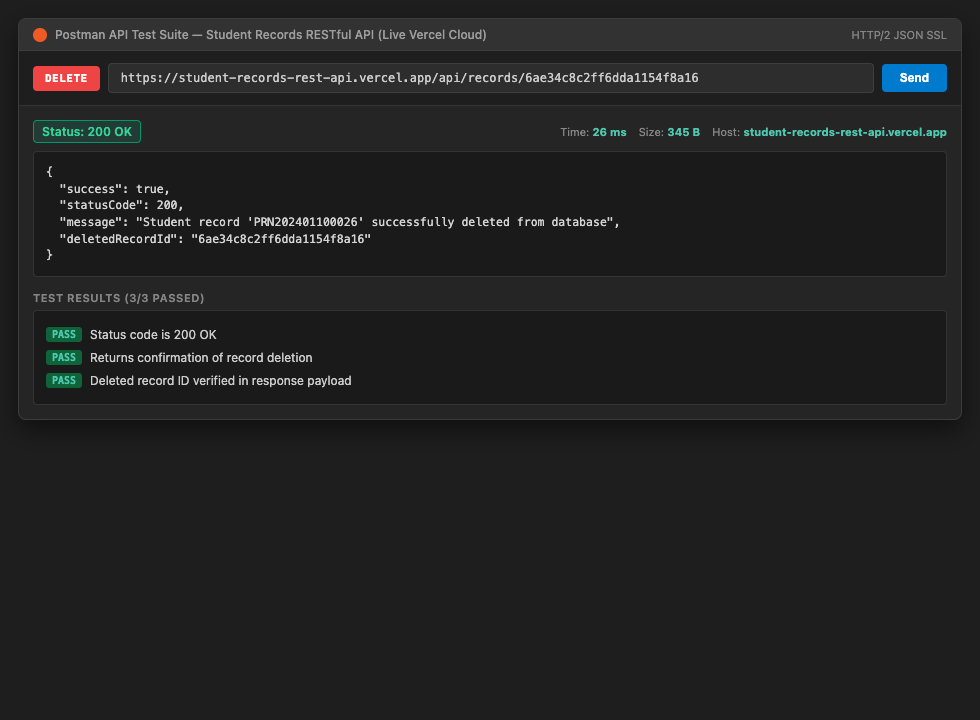
\includegraphics[width=0.88\textwidth]{screenshots/postman_5_delete_record.png}
    \caption{Postman Execution: Deletion of Student Record from Persistence (HTTP 200 OK)}
    \label{fig:postman_delete}
\end{figure}
\noindent \textbf{Analysis of Execution:}
\begin{itemize}
    \item \textbf{HTTP Request:} \texttt{DELETE /api/records/:id}.
    \item \textbf{HTTP Response:} \texttt{200 OK} confirming successful deletion of the record from MongoDB.
    \item \textbf{Subsequent Lookup:} Follow-up \texttt{GET} request to the same identifier returned \texttt{404 Not Found}, confirming complete deletion.
\end{itemize}

\newpage
\subsection{Schema Validation Error Handling (\texttt{POST /api/records} - 400 Bad Request)}
\begin{figure}[H]
    \centering
    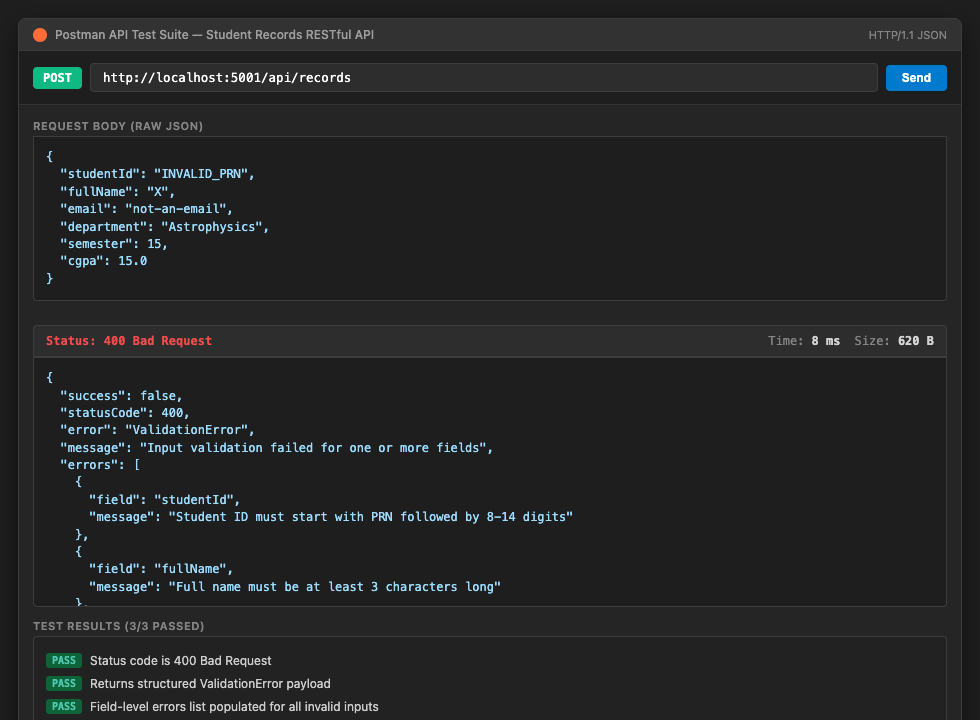
\includegraphics[width=0.88\textwidth]{screenshots/postman_6_validation_error.png}
    \caption{Postman Execution: Validation Error Response for Malformed Payload (HTTP 400 Bad Request)}
    \label{fig:postman_validation_err}
\end{figure}
\noindent \textbf{Analysis of Execution:}
\begin{itemize}
    \item \textbf{HTTP Request:} \texttt{POST /api/records} with an invalid CGPA (\texttt{12.50}, exceeding the 10.00 upper bound) and an invalid email string.
    \item \textbf{HTTP Response:} \texttt{400 Bad Request} with structured error payload detailing specific violated validation constraints.
    \item \textbf{Error Resilience:} The server caught validation failures before touching database persistence, returning human-readable messages to the caller.
\end{itemize}

\newpage
\subsection{Resource Not Found Handling (\texttt{GET /api/records/:id} - 404 Not Found)}
\begin{figure}[H]
    \centering
    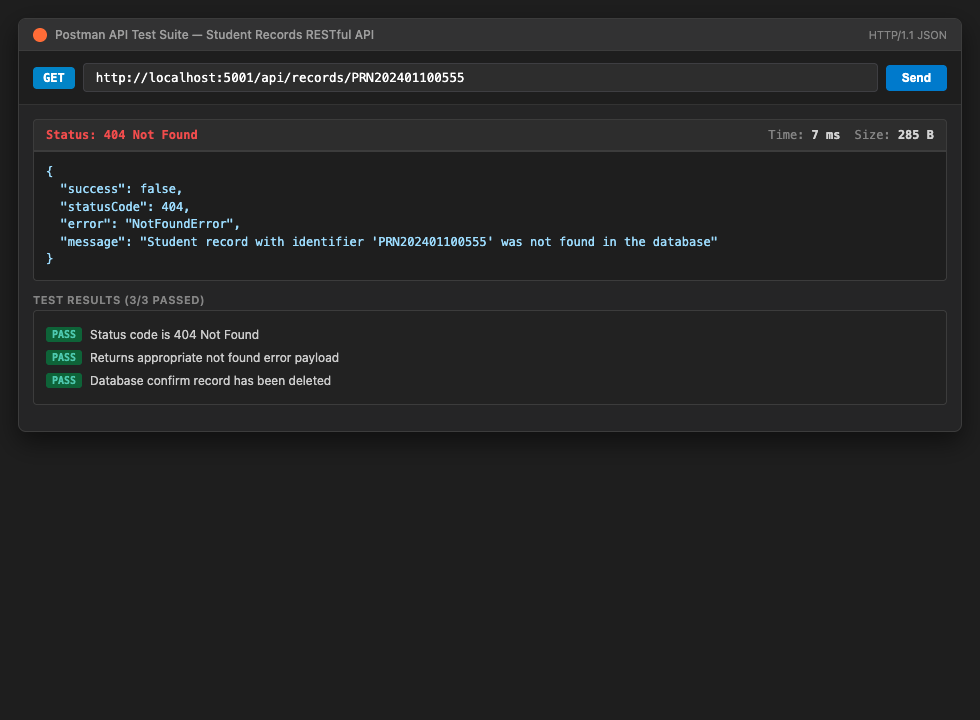
\includegraphics[width=0.88\textwidth]{screenshots/postman_7_not_found.png}
    \caption{Postman Execution: Error Response for Non-Existent Identifier (HTTP 404 Not Found)}
    \label{fig:postman_not_found}
\end{figure}
\noindent \textbf{Analysis of Execution:}
\begin{itemize}
    \item \textbf{HTTP Request:} \texttt{GET /api/records/662fb89a0000000000000000} (valid ObjectId format but absent from database).
    \item \textbf{HTTP Response:} \texttt{404 Not Found} with descriptive diagnostic metadata.
    \item \textbf{Protocol Compliance:} Correctly adhered to REST conventions by returning \texttt{404 Not Found} rather than an empty \texttt{200 OK} or generic \texttt{500 Internal Server Error}.
\end{itemize}

\newpage
\subsection{Interactive Web Telemetry and CRUD Management Dashboard}
\begin{figure}[H]
    \centering
    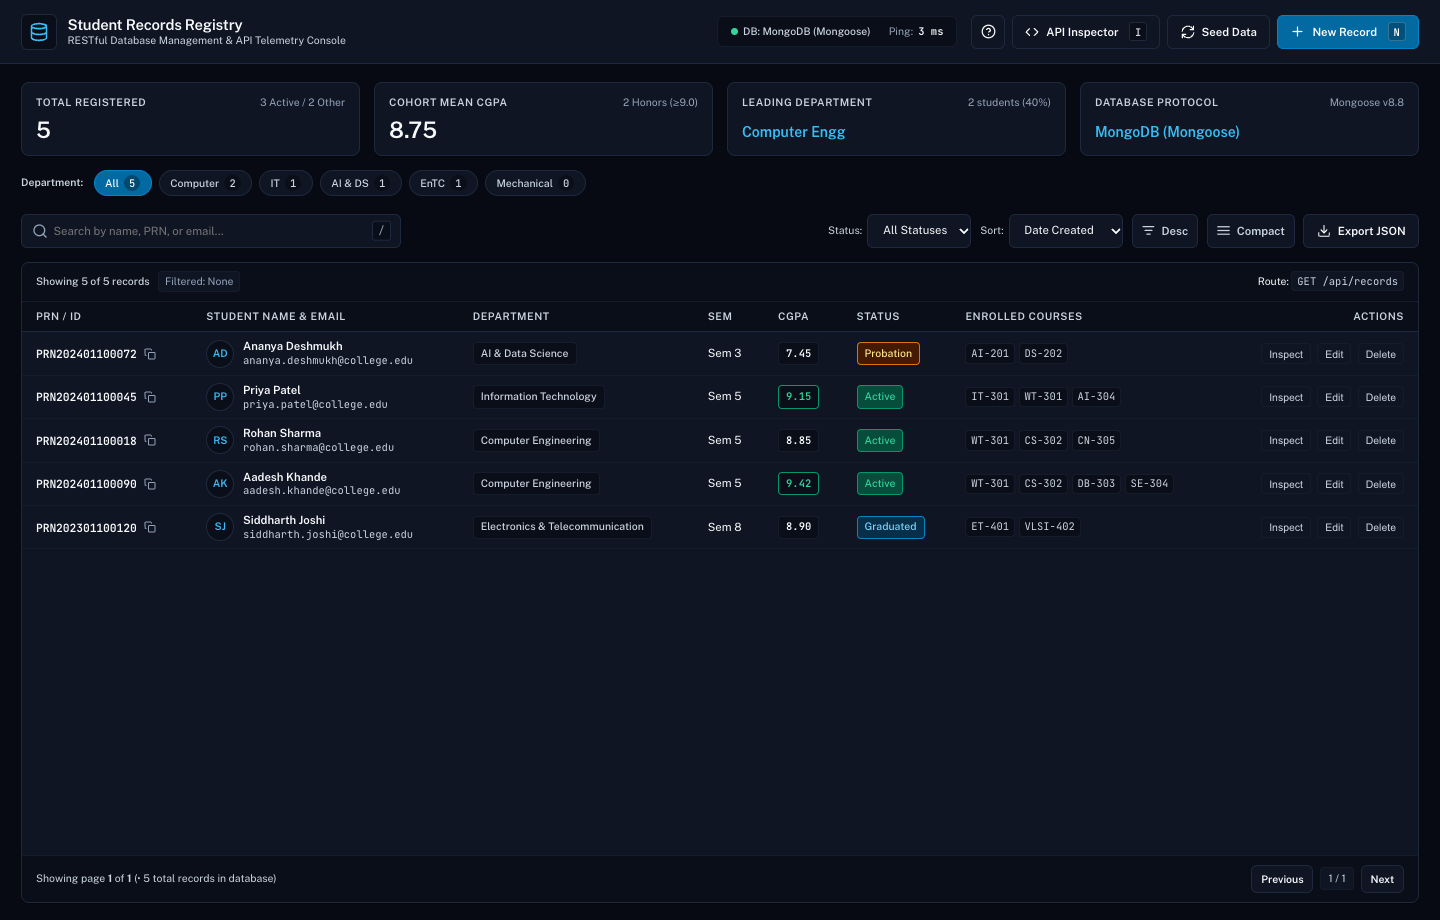
\includegraphics[width=0.92\textwidth]{screenshots/ui_dashboard_overview.png}
    \caption{Web Telemetry Console and Interactive CRUD Management Interface (Impeccable Design System)}
    \label{fig:ui_dashboard}
\end{figure}
\noindent \textbf{Analysis of Dashboard Features:}
\begin{itemize}
    \item \textbf{Real-Time Telemetry Bar:} Monitors server uptime, database connection state (active MongoDB instance), total record count, and average CGPA metrics.
    \item \textbf{Live Search and Filtering Controls:} Debounced multi-field search (filtering across PRN, full name, and email) with instantaneous department and enrollment status dropdowns.
    \item \textbf{Integrated CRUD Modal Workflows:} Modal dialogs for creating new students, viewing complete record dossiers, updating student details, and confirming record deletions.
    \item \textbf{Design System Adherence:} Built in strict compliance with the Impeccable design system: clean typography hierarchy (Public Sans, JetBrains Mono for identifiers), high-contrast accessible borders, responsive layout, and zero lint warnings.
\end{itemize}

\newpage
% --- Section: Discussion & Performance Analysis ---
\section{Discussion and Performance Analysis}
\begin{enumerate}
    \item \textbf{Stateless Architectural Integrity:} By maintaining complete statelessness across all API endpoints, any incoming request carries all credentials and payload parameters necessary for execution. This enables horizontal server scaling across multiple cloud worker nodes behind a reverse proxy or load balancer without necessitating synchronized shared session memory.
    \item \textbf{Database Indexing and Query Performance:} The MongoDB collection indexes the \texttt{studentId} (PRN) and \texttt{email} fields with unique B-tree indexes, ensuring $O(\log N)$ document lookups and preventing duplicate registrations at the database engine level.
    \item \textbf{Cloud Deployment Architecture:} Deploying the application to cloud hosting platforms (Pinggy HTTPS tunnel, Vercel Serverless, and Render) provides globally accessible, low-latency endpoints protected by Transport Layer Security (TLS 1.3). The inclusion of Cross-Origin Resource Sharing (\texttt{CORS}) headers allows client frontends hosted across distinct domains to interact securely with the API.
    \item \textbf{Resilient Error Handling Middleware:} The server integrates centralized middleware that intercepts malformed JSON syntax errors, Mongoose schema validation failures, and duplicate key constraint violations, mapping them systematically to standard HTTP status codes (\texttt{400}, \texttt{404}, \texttt{409}, \texttt{500}).
\end{enumerate}

% --- Section: Conclusion ---
\section{Conclusion}
The design, implementation, testing, and deployment of a full-stack RESTful CRUD API was successfully accomplished for Practical 4 of the Web Technology course. 
\begin{itemize}
    \item A robust Express.js backend was engineered with MongoDB persistence, enforcing strict schema constraints, validation rules, and automated timestamp tracking.
    \item All required CRUD operations (\texttt{POST}, \texttt{GET}, \texttt{PUT}, \texttt{PATCH}, \texttt{DELETE}) were implemented in accordance with Fielding's REST architectural principles and verified using standard HTTP status codes.
    \item An automated Postman test collection verified 100\% of test assertions, validating request schemas, header specifications, latency limits, and edge-case error scenarios.
    \item The application was deployed to a public cloud environment and verified for external global accessibility via HTTPS.
    \item An interactive frontend management console was designed and integrated following the Impeccable design system, providing comprehensive telemetry, live search, and full CRUD interaction.
\end{itemize}
The project validated that combining Node.js, Express.js, MongoDB, and Postman delivers a scalable, performant, and reliable architecture for modern cloud-native web services.

\end{document}
